\documentclass[tikz,border=10pt]{standalone}
% Shared look for every TikZ diagram. Load with % Shared look for every TikZ diagram. Load with % Shared look for every TikZ diagram. Load with \input{../../tools/tikz-style.tex}
\usepackage[T1]{fontenc}
\usepackage{lmodern}
\renewcommand{\sfdefault}{lmr}  % diagrams use the same serif as the text
\usetikzlibrary{arrows.meta, positioning, shapes.geometric, calc, fit, backgrounds}
\definecolor{cblue}{HTML}{4C78A8}
\definecolor{corange}{HTML}{F58518}
\definecolor{cgreen}{HTML}{54A24B}
\definecolor{cred}{HTML}{E45756}
\definecolor{cpurple}{HTML}{B279A2}
\definecolor{cgrey}{HTML}{6B6B6B}
\tikzset{
  every picture/.style={font=\sffamily, line width=1.2pt},
  box/.style={draw=#1, fill=#1!12, rounded corners=4pt, align=center, inner sep=7pt, minimum height=1.1cm},
  box/.default=cgrey,
  arrow/.style={-{Stealth[length=3mm]}, draw=cgrey, line width=1.4pt},
  title/.style={font=\sffamily\bfseries\Large},
  note/.style={font=\sffamily\small, text=cgrey, align=center},
}
\AtBeginDocument{\hyphenpenalty=10000 \exhyphenpenalty=10000}

\usepackage[T1]{fontenc}
\usepackage{lmodern}
\renewcommand{\sfdefault}{lmr}  % diagrams use the same serif as the text
\usetikzlibrary{arrows.meta, positioning, shapes.geometric, calc, fit, backgrounds}
\definecolor{cblue}{HTML}{4C78A8}
\definecolor{corange}{HTML}{F58518}
\definecolor{cgreen}{HTML}{54A24B}
\definecolor{cred}{HTML}{E45756}
\definecolor{cpurple}{HTML}{B279A2}
\definecolor{cgrey}{HTML}{6B6B6B}
\tikzset{
  every picture/.style={font=\sffamily, line width=1.2pt},
  box/.style={draw=#1, fill=#1!12, rounded corners=4pt, align=center, inner sep=7pt, minimum height=1.1cm},
  box/.default=cgrey,
  arrow/.style={-{Stealth[length=3mm]}, draw=cgrey, line width=1.4pt},
  title/.style={font=\sffamily\bfseries\Large},
  note/.style={font=\sffamily\small, text=cgrey, align=center},
}
\AtBeginDocument{\hyphenpenalty=10000 \exhyphenpenalty=10000}

\usepackage[T1]{fontenc}
\usepackage{lmodern}
\renewcommand{\sfdefault}{lmr}  % diagrams use the same serif as the text
\usetikzlibrary{arrows.meta, positioning, shapes.geometric, calc, fit, backgrounds}
\definecolor{cblue}{HTML}{4C78A8}
\definecolor{corange}{HTML}{F58518}
\definecolor{cgreen}{HTML}{54A24B}
\definecolor{cred}{HTML}{E45756}
\definecolor{cpurple}{HTML}{B279A2}
\definecolor{cgrey}{HTML}{6B6B6B}
\tikzset{
  every picture/.style={font=\sffamily, line width=1.2pt},
  box/.style={draw=#1, fill=#1!12, rounded corners=4pt, align=center, inner sep=7pt, minimum height=1.1cm},
  box/.default=cgrey,
  arrow/.style={-{Stealth[length=3mm]}, draw=cgrey, line width=1.4pt},
  title/.style={font=\sffamily\bfseries\Large},
  note/.style={font=\sffamily\small, text=cgrey, align=center},
}
\AtBeginDocument{\hyphenpenalty=10000 \exhyphenpenalty=10000}

\begin{document}
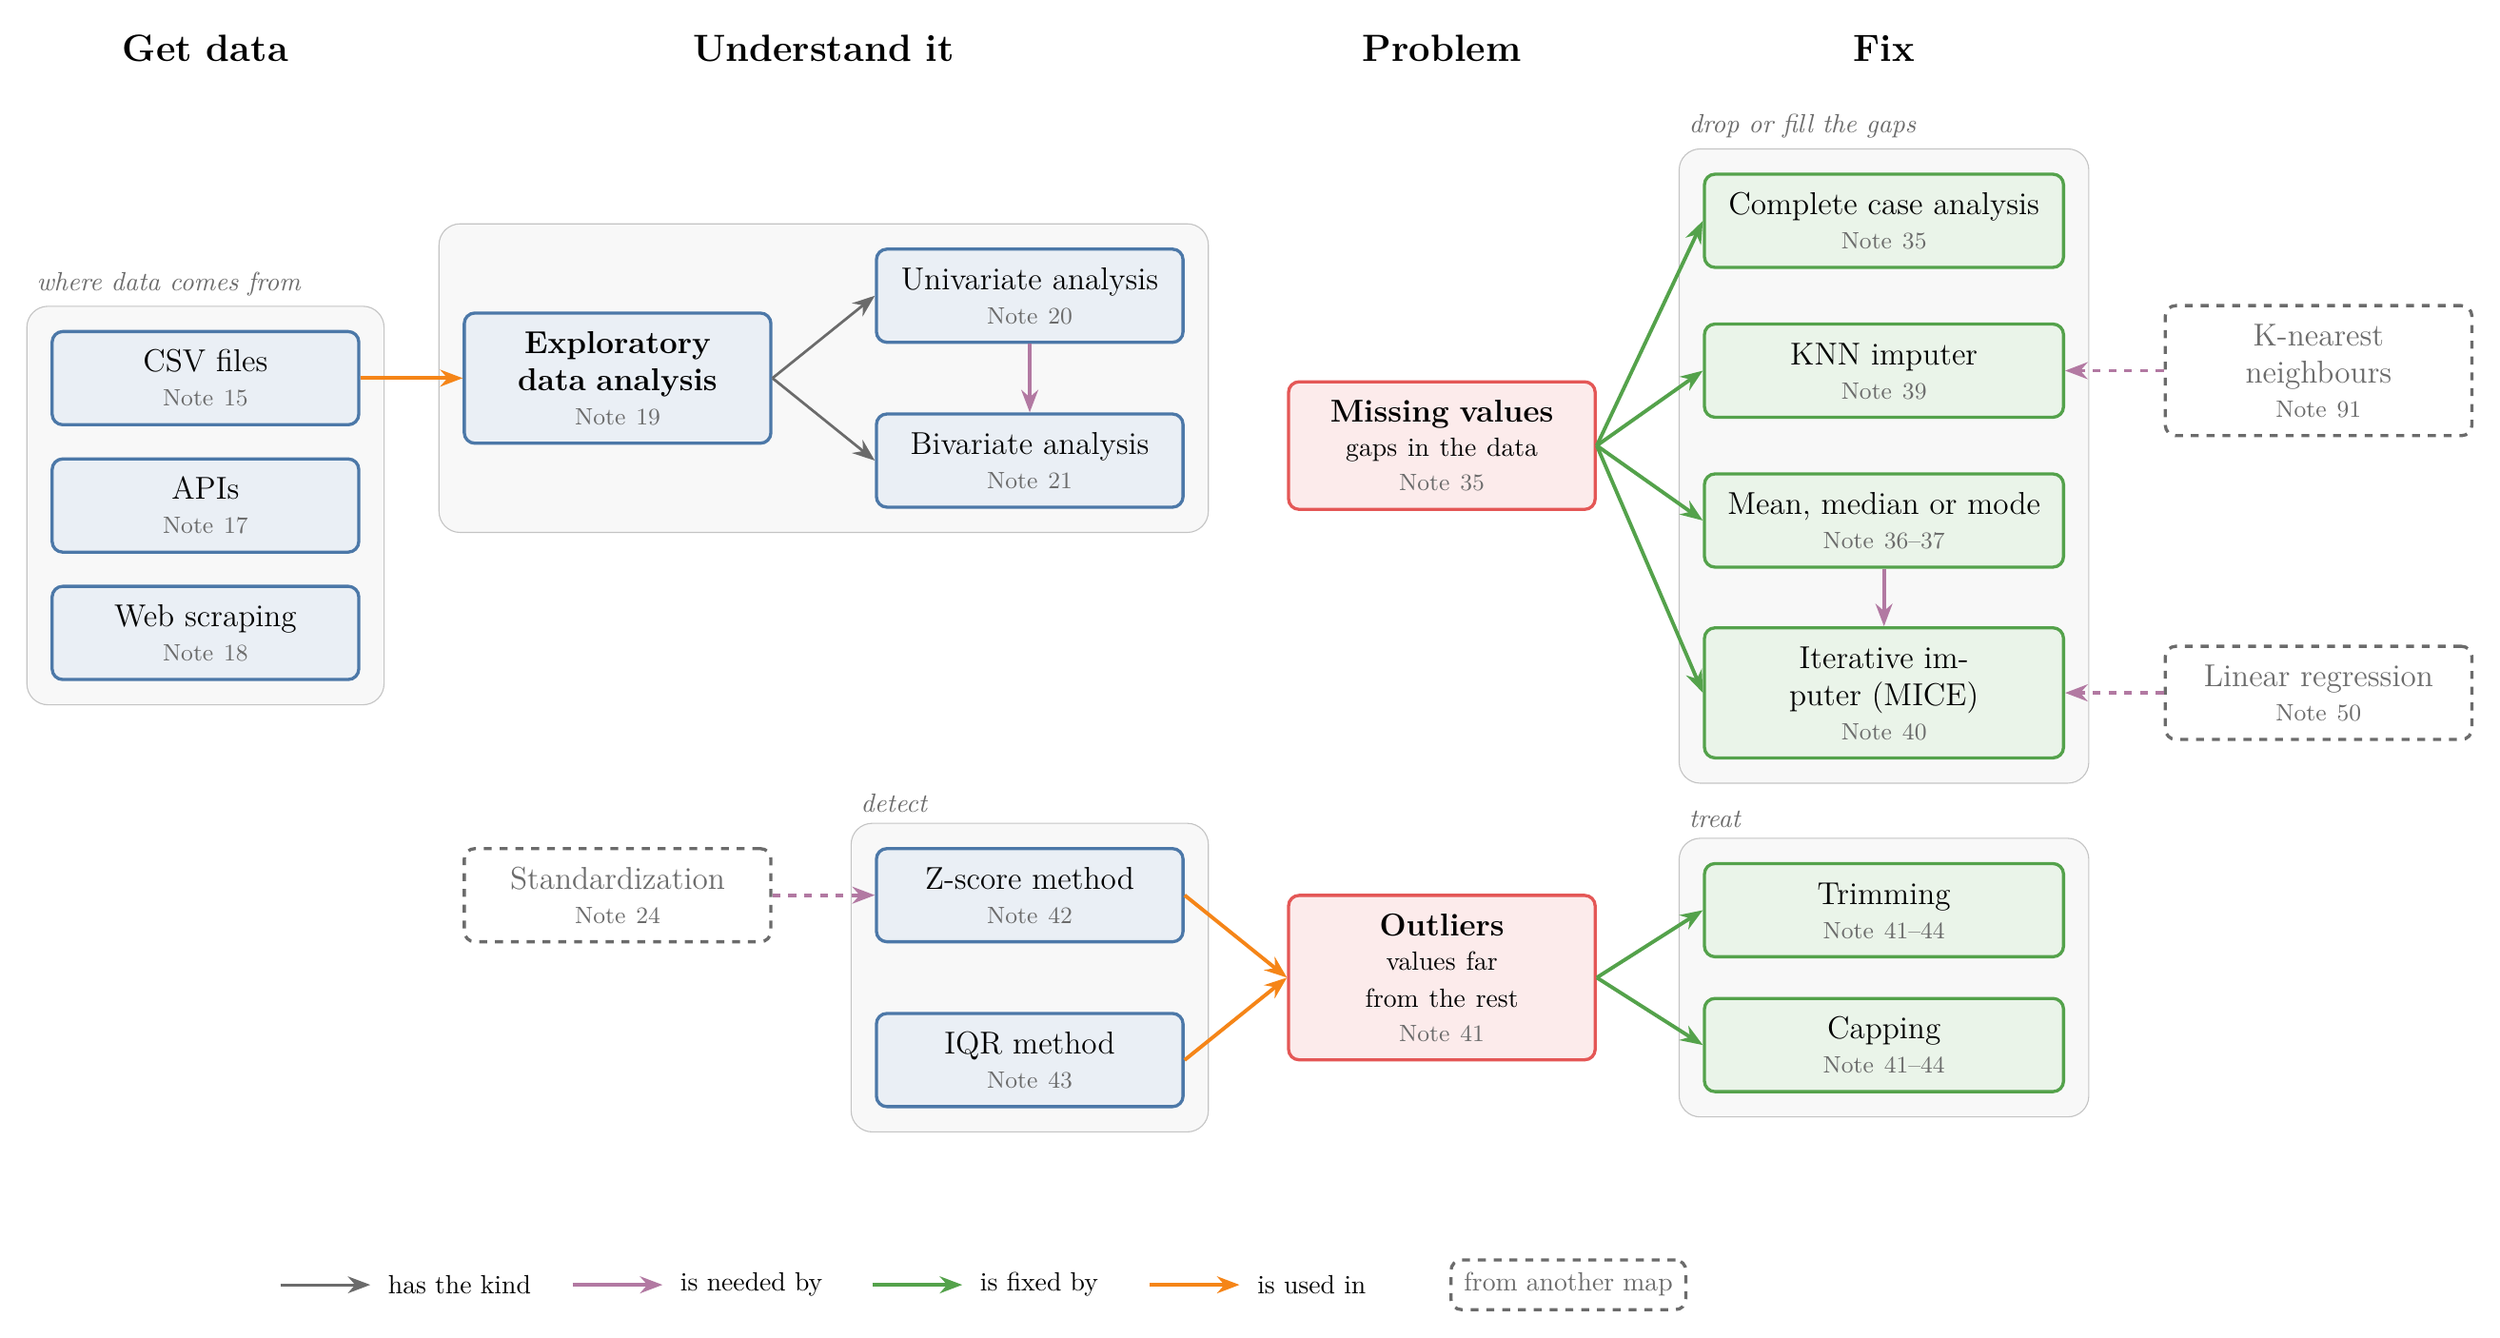
\begin{tikzpicture}[
    every node/.append style={font=\sffamily\large},
    dstep/.style={box=cblue, text width=3.6cm},
    prob/.style={box=cred, text width=3.6cm},
    fix/.style={box=cgreen, text width=4.3cm},
    prev/.style={draw=cgrey, dashed, rounded corners=4pt, align=center, inner sep=7pt, text=cgrey, text width=3.6cm, minimum height=1.1cm},
    group/.style={draw=cgrey!40, fill=cgrey!5, rounded corners=8pt, inner sep=9pt},
    gname/.style={font=\sffamily\normalsize\itshape, text=cgrey, anchor=south west},
    kindof/.style={arrow, draw=cgrey, line width=1pt},
    needs/.style={arrow, draw=cpurple},
    fixes/.style={arrow, draw=cgreen},
    usedin/.style={arrow, draw=corange},
  ]
  \newcommand{\nt}[1]{\\[-1pt]{\small\color{cgrey}Note #1}}
  \node[title] at (0,11.9)    {Get data};
  \node[title] at (8.25,11.9) {Understand it};
  \node[title] at (16.5,11.9) {Problem};
  \node[title] at (22.4,11.9)   {Fix};

  % get data
  \node[dstep] (csv)    at (0,7.5) {CSV files\nt{15}};
  \node[dstep] (api)    at (0,5.8) {APIs\nt{17}};
  \node[dstep] (scrape) at (0,4.1) {Web scraping\nt{18}};

  % understand data
  \node[dstep] (eda) at (5.5,7.5) {\textbf{Exploratory}\\\textbf{data analysis}\nt{19}};
  \node[dstep] (uni) at (11,8.6)  {Univariate analysis\nt{20}};
  \node[dstep] (bi)  at (11,6.4)  {Bivariate analysis\nt{21}};
  \draw[usedin] (csv) -- (eda);
  \draw[kindof] (eda.east) -- (uni.west);
  \draw[kindof] (eda.east) -- (bi.west);
  \draw[needs] (uni) -- (bi);

  % clean: missing values
  \node[prob] (miss) at (16.5,6.6) {\textbf{Missing values}\\[-1pt]{\normalsize gaps in the data}\nt{35}};
  \node[fix] (cc)   at (22.4,9.6) {Complete case analysis\nt{35}};
  \node[fix] (knni) at (22.4,7.6) {KNN imputer\nt{39}};
  \node[fix] (simp) at (22.4,5.6) {Mean, median or mode\nt{36--37}};
  \node[fix] (mice) at (22.4,3.3) {Iterative imputer (MICE)\nt{40}};
  \foreach \f in {cc, knni, simp, mice} \draw[fixes] (miss.east) -- (\f.west);
  \draw[needs] (simp) -- (mice);
  \node[prev] (knn) at (28.2,7.6) {K-nearest neighbours\nt{91}};
  \node[prev] (lr)  at (28.2,3.3) {Linear regression\nt{50}};
  \draw[needs, dashed] (knn) -- (knni);
  \draw[needs, dashed] (lr) -- (mice);

  % clean: outliers
  \node[prob] (out) at (16.5,-0.5) {\textbf{Outliers}\\[-1pt]{\normalsize values far from the rest}\nt{41}};
  \node[dstep] (z)   at (11,0.6)  {Z-score method\nt{42}};
  \node[dstep] (iqr) at (11,-1.6) {IQR method\nt{43}};
  \node[fix] (trim) at (22.4,0.4)  {Trimming\nt{41--44}};
  \node[fix] (cap)  at (22.4,-1.4) {Capping\nt{41--44}};
  \draw[usedin] (z.east) -- (out.west);
  \draw[usedin] (iqr.east) -- (out.west);
  \draw[fixes] (out.east) -- (trim.west);
  \draw[fixes] (out.east) -- (cap.west);
  \node[prev] (std) at (5.5,0.6) {Standardization\nt{24}};
  \draw[needs, dashed] (std) -- (z);

  \begin{scope}[on background layer]
    \node[group, fit=(csv) (scrape)] (g1) {};
    \node[group, fit=(eda) (uni) (bi)] (g2) {};
    \node[group, fit=(cc) (mice)] (g3) {};
    \node[group, fit=(z) (iqr)] (g4) {};
    \node[group, fit=(trim) (cap)] (g5) {};
  \end{scope}
  \node[gname] at (g1.north west) {where data comes from};
  \node[gname] at (g3.north west) {drop or fill the gaps};
  \node[gname] at (g4.north west) {detect};
  \node[gname] at (g5.north west) {treat};

  % legend
  \begin{scope}[shift={(1,-4.6)}, every node/.style={font=\sffamily, anchor=west}]
    \draw[kindof] (0,0) -- (1.2,0);   \node at (1.3,0) {has the kind};
    \draw[needs] (3.9,0) -- (5.1,0);  \node at (5.2,0) {is needed by};
    \draw[fixes] (7.9,0) -- (9.1,0);  \node at (9.2,0) {is fixed by};
    \draw[usedin] (11.6,0) -- (12.8,0); \node at (12.9,0) {is used in};
    \node[draw=cgrey, dashed, rounded corners=4pt, inner sep=5pt, text=cgrey, anchor=west] at (15.6,0) {from another map};
  \end{scope}
\end{tikzpicture}
\end{document}
